\chapter{Security, Operations, and Cost}
\section{Security Design}
The public browser interfaces use HTTPS through CloudFront and API Gateway. The API authenticates application users and applies role and classroom access checks. Passwords are hashed, and student sessions do not grant access to fault injection. The recovery cockpit requires a separate administrator control token.

Network policy restricts application ingress to the router/verifier security group on port 8000. The deployment does not open inbound SSH; Systems Manager supports instance management. Backend traffic within the VPC uses HTTP in the prototype, which makes the private network boundary significant. Additional service-to-service transport protection is a production hardening requirement.

Runtime service roles provide AWS credentials to EC2 and Lambda. Bootstrap configuration is stored in an encrypted Systems Manager parameter, and the application bundle is retrieved from a private S3 bucket. Private runtime files, deployment outputs, and Terraform state must be protected because they can contain operational secrets.
\section{Separation of Service Permissions}
The application role can access the table for permitted application operations, including conditional checks on the active record. Explicit policy restrictions prevent it from writing the control and audit namespaces. The control function manages the active writer and instance operations, while the reconciler owns its bounded audit-processing responsibility.

The monitor is configured without the fault-control token. The workflow role invokes the functions needed for the recovery sequence. This distribution limits the authority of a component that only needs to observe or forward requests. The model concerns service permissions; human team-member access remains managed through the AWS project experience.
\section{Threat and Failure Considerations}

\begin{table}[H]\centering\small
\caption{Selected risks and implemented controls}\label{tab:risks}
\begin{tabularx}{\textwidth}{@{}L{41mm}Y@{}}\toprule
\textbf{Risk or failure} & \textbf{Control and remaining boundary}\\\midrule
Unauthorised fault action & Separate administrator token; credential protection remains essential\\
Forged or obsolete writer context & Private ingress plus database-enforced backend/epoch condition\\
Concurrent recovery actions & Incident lease, expected-state conditions, retry-safe promotion\\
Changed answers under one request ID & Scope and payload binding with conflict rejection\\
Misleading healthy process & Deep readiness and healthy-standby confirmation\\
Interrupted audit processing & Atomic outbox and conditional reconciliation\\
Private data in operational artifacts & Private state/output files; synthetic demonstration data\\
Shared regional dependency failure & Suppress unsafe promotion; outside the demonstrated recovery scope\\\bottomrule
\end{tabularx}\end{table}

The prototype is not presented as an institutional examination service ready for unrestricted use. Formal privacy review, retention policy, broader abuse controls, external security testing, backup/restore exercises, and operational ownership would be needed before using real examination data at scale.
\section{Operational Lifecycle}
Development and most rehearsals can use local mode. Cloud resources are enabled for bounded demonstration windows. The supported lifecycle is deploy, resume, verify both backends, perform the controlled scenario, capture the outcome, and pause the stack.

Before a cloud deployment, the selected Region is confirmed through AWS Settings, under View all projects, Overview, Additional Info, Region. The supported Terraform configuration validates Sydney and rejects another regional value. The project plan and current spend status are checked through AWS Settings and the plan API before resources are started. The recorded rehearsal used the Free plan; this historical fact does not establish a later credit balance.

Pause stops the EC2 instances and disables the monitoring schedule. Existing executions can finish, and retained disks, data, logs, or objects can continue to consume credits. Destruction is a separate action that removes persistent data as well as compute, so required synthetic results must first be retained deliberately.
\section{Monitoring Delay and Activity Models}
Monitoring frequency creates a direct trade-off between nominal detection delay and recurring work. The implemented scheduled monitor runs once per minute. Three confirmation probes have two five-second gaps, so even a fault discovered immediately requires a nominal ten seconds of confirmation spacing. Figure~\ref{fig:monitor-delay} explores one-, two-, and five-minute schedules; only the one-minute rate is the current deployment.

Let $S$ be the schedule period in seconds, $\phi\in[0,1]$ the fault's position within a schedule cycle, $p=3$ the number of probes, and $\delta=5$ seconds their spacing. An idealised model is
\begin{equation}
D_{\mathrm{nominal}}(S,\phi)=S(1-\phi)+(p-1)\delta.
\end{equation}
This excludes probe duration, schedule jitter, invocation latency, and subsequent workflow work. It is a planning model rather than a prediction or a bound on actual recovery. With uniformly distributed fault phase, its expected value is $S/2+10$: 40, 70, and 160 seconds for the three schedules.

\begin{figure}[htbp]\centering
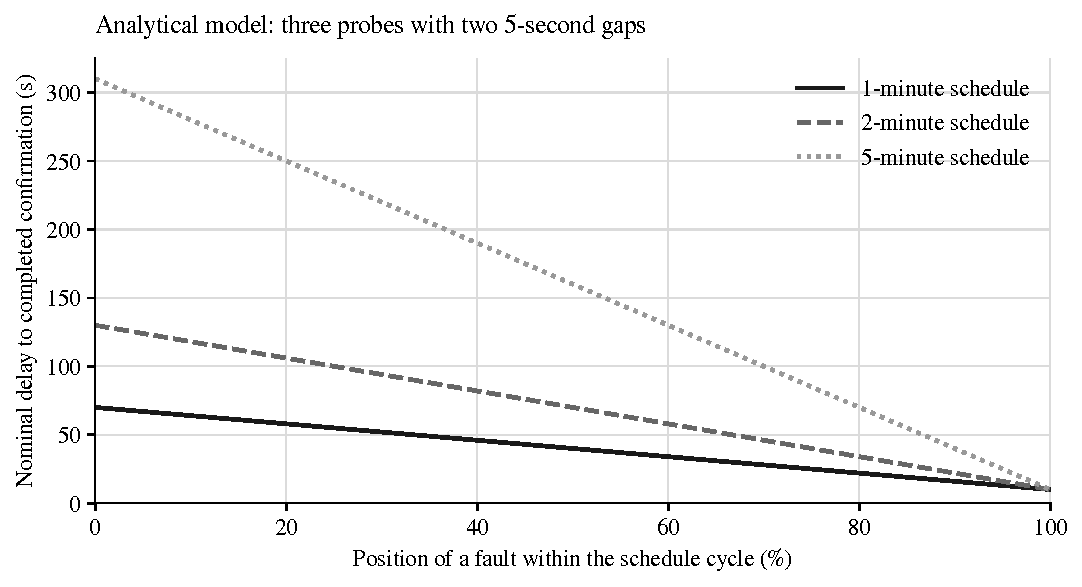
\includegraphics[width=\textwidth]{figures/monitor-phase-model.pdf}
\caption[Analytical monitoring and confirmation delay]{Analytical confirmation-delay scenarios, not measured performance. Faults just after a scheduled check wait almost a full cycle before confirmation can begin.}\label{fig:monitor-delay}
\end{figure}

For $h$ hours with monitoring enabled, the nominal scheduled activity is
\begin{equation}
N_{\mathrm{scheduled}}=\frac{3600h}{S}.
\end{equation}
At the implemented one-minute rate, a two-hour rehearsal produces 120 nominal monitor triggers and continuous daily operation produces 1,440. These counts exclude retries, manual invocations, and recovery workflow calls. They cannot be multiplied by a single unit price to obtain the entire cloud bill.

\begin{figure}[htbp]\centering
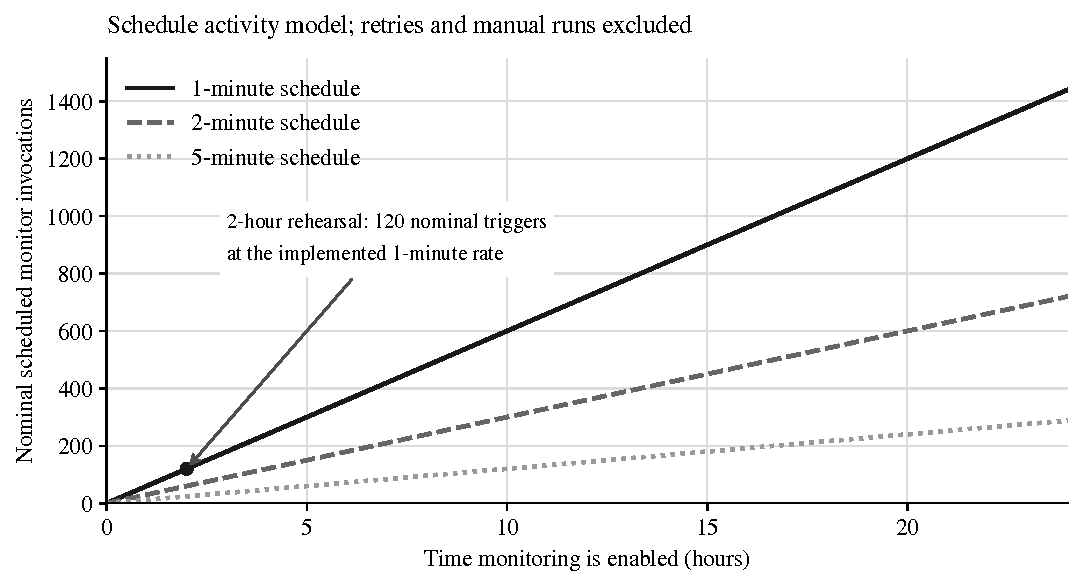
\includegraphics[width=\textwidth]{figures/monitor-activity-model.pdf}
\caption[Analytical scheduled monitoring activity]{Analytical monitoring activity against enabled hours. A slower schedule reduces recurring calls while increasing the phase-dependent wait shown in Figure~\ref{fig:monitor-delay}.}\label{fig:monitor-activity}
\end{figure}

The appropriate policy depends on the acceptable interruption and the cost of a false promotion. For this small demonstration, three probes suppress a short-lived fault and avoid reacting to a single failed request. Lower latency would require changing and validating the detection path, not simply claiming that public health recovery is instantaneous. Repeated trials with randomised fault phase should precede any production RTO claim.

\FloatBarrier
\section{Cost Model}
The major cost drivers are the two EC2 instances, their public IPv4 addresses while assigned, retained EBS volumes, DynamoDB operations and storage, Lambda invocations, API Gateway requests, workflow transitions, S3 objects, CloudFront delivery, and logs. Gateway VPC endpoints for S3 and DynamoDB have no additional endpoint charge~\cite{aws-endpoints}. The design avoids fixed NAT gateway and load-balancer resources.

A planning model separates active runtime from retained storage:
\begin{equation}
C_{\mathrm{period}}=2h(P_{\mathrm{EC2}}+P_{\mathrm{IPv4}})+C_{\mathrm{EBS}}+C_{\mathrm{requests}}+C_{\mathrm{storage}}+C_{\mathrm{delivery/logs}},
\end{equation}
where $h$ is the number of hours that both application instances are running. Rates depend on the selected Region and current pricing. This expression identifies cost drivers; it is not a fixed quotation or a guarantee that credits cover the deployment. Current EC2, VPC, and EBS rates should be checked for the actual rehearsal period~\cite{aws-ec2-price,aws-vpc-price,aws-ebs-price}.

The HTTP API stage is configured for a rate of three requests per second and burst capacity of six. No reserved Lambda concurrency is allocated. These values bound the demonstration and must not be treated as a capacity plan for a large cohort. Pause/resume, limited log retention, local rehearsal, and deterministic builds support efficient use of the available resources.
\section{Alignment with Cloud Architecture Principles}
The AWS Well-Architected Framework describes six pillars~\cite{aws-wellarchitected}. Table~\ref{tab:pillars} maps the implementation to those themes without claiming a formal framework review.

\begin{table}[H]\centering\small
\caption{Relationship to the Well-Architected pillars}\label{tab:pillars}
\begin{tabularx}{\textwidth}{@{}L{38mm}Y@{}}\toprule
\textbf{Pillar} & \textbf{Relevant project decision}\\\midrule
Operational excellence & Observable events, documented runbook, reproducible local checks\\
Security & Restricted ingress, service roles, separate operational token\\
Reliability & Standby verification, atomic fencing, receipt replay, outbox recovery\\
Performance efficiency & Bounded functions, timeouts, and explicit small-demo traffic limits\\
Cost optimisation & Local-first rehearsal, pause controls, absence of fixed NAT/load-balancer resources\\
Sustainability & Stop idle compute and retain only necessary demonstration artifacts\\\bottomrule
\end{tabularx}\end{table}

